\documentclass[9pt]{article}
\usepackage[utf8]{inputenc}
\usepackage{amsmath,amsthm,amsfonts,amssymb,amscd}
\usepackage{multirow,booktabs}
\usepackage{enumitem}
\usepackage{fancyhdr}
\usepackage{mathrsfs}
\usepackage{wrapfig}
\usepackage{setspace}
\usepackage{calc}
\usepackage{subfig}
\usepackage{multicol}
\usepackage{cancel}
\usepackage[retainorgcmds]{IEEEtrantools}
\usepackage{framed}
\usepackage[most]{tcolorbox}
\usepackage{tikz}
\usepackage{geometry}
\geometry{
	a4paper,
	total={170mm,257mm},
	left=20mm,
	top=20mm,
}
\title{Electric Potential}
\author{Aaron G.K.}

\begin{document}
	\maketitle
	\begin{center}
		\section*{Electric Potential and Potential Energy}	
	\end{center}
	When a free positive charge  q  is accelerated by an electric field, it is given kinetic energy. The process is analogous to an object being accelerated by a gravitational field. It is as if the charge is going down an electrical hill where its electric potential energy is converted to kinetic energy. 
	\begin{center}
		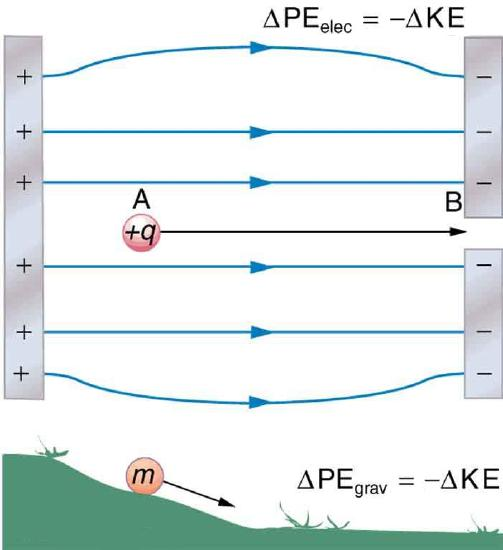
\includegraphics[scale=0.5]{pe_analogy}
	\end{center}
	The electrostatic force is conservative, which means that the work done on q is independent of the path taken(it also conserves the mechanical energy). This is exactly analogous to the gravitational force in the absence of dissipative forces such as friction. When a force is conservative, it is possible to define a potential energy associated with the force, and it is usually easier to deal with the potential energy (because it depends only on position) than to calculate the work directly. \\ \\
	We use the letters PE to denote electric potential energy, which has units of joules (J). The change in potential energy, $\varDelta$PE, is crucial, since the work done by a conservative force is the negative of the change in potential energy; that is, W=$-\varDelta$PE. For example, work W done to accelerate a positive charge from rest is positive and results from a loss in PE, or a negative $\varDelta$PE. There must be a minus sign in front of $\varDelta$PE to make W positive. PE can be found at any point by taking one point as a reference and calculating the work needed to move a charge to the other point. \\ \\
	We can show that the potential energy is equal to the work done as follows. We know that the mechanical energy is conserved in the presence of conservative forces. 
	$$\text{ME}_i=\text{ME}_f$$
	$$\text{KE}_i+\text{PE}_i=\text{KE}_f+\text{PE}_f$$
	We can rearrange the above equation as follows:
	$$\text{KE}_i-\text{KE}_f=\text{PE}_f-\text{PE}_i$$
	$$-\Delta\text{KE}=\Delta\text{PE}$$
	According to the work-kinetic energy theorem, the change in kinetic energy is the work done. As such, we have the following:
	$$-\Delta\text{W}=\Delta\text{PE}$$
	$$\Delta\text{PE}=-\Delta\text{W}$$
	W=$-\Delta$PE . For example, work  W  done to accelerate a positive charge from rest is positive and results from a loss in PE, or a negative  $\Delta$PE  there must be a negative sign in front of  $\Delta$ PE  to make  W  positive. PE can be found at any point by taking one point as a reference and calculating the work needed to move a charge to the other point.\\ \\
	We know that the potential energy is the work done by the conservative forces. Calculating the work directly is generally difficult, since  the direction and magnitude of F can be complex for multiple charges, for odd-shaped objects, and along arbitrary paths. But we do know that, since  F=qE , the work, and hence  $\Delta$PE , is proportional to the test charge  q. To have a physical quantity that is independent of test charge, we define electric potential  V to be the potential energy per unit charge:
	$$V=\dfrac{\text{PE}}{q}$$
	Since PE is proportional to  q, the dependence on  q  cancels. Thus  V  does not depend on  q. The change in potential energy  $\Delta$PE  is crucial, and so we are concerned with the difference in potential $\Delta$V  between two points, called the \textit{potential difference} or \textit{voltage}. \\ \\
	Thus, for two arbitrary points A \& B near a source charge, the potential difference is given by:
	$$\Delta V =V_{B}-V_{A}=\dfrac{\Delta \text{PE}}{q}.$$ 
	The SI unit of V is Volt, after Alessandro Volta. It is important to note that $1 \text{V}=1\dfrac{\text{J}}{\text{C}}$ \\ 
	\subsubsection*{Important note on voltage}
	The term \textbf{voltage} is the common name for potential difference. Keep in mind that whenever we say voltage , it is understood to be the potential difference between two points. For example, every battery has two terminals, and its voltage is the potential difference between them. \textit{\textbf{More fundamentally, the point you choose to be zero volts is arbitrary}}. This is analogous to the fact that gravitational potential energy has an arbitrary zero, such as the ground from which we measure the height from. \\ \\
	It is also imperative to note that voltage is not the same as energy. Voltage is the energy per unit charge. Thus a remote control battery and a flashlight battery can both have the same voltage (the same potential difference between battery terminals), yet one stores much more energy than the other since $\Delta$PE=q$\Delta$V. The car battery can move more charge than the motorcycle battery, although could be 1.5 V batteries.
	\subsubsection*{Relationship with Electric Field}
	For a simple and uniform electric field, we can relate the electric field to the potential. For example, a uniform electric field E is produced by placing a potential difference $\Delta$V across two parallel metal plates as shown below.
	\begin{center}
		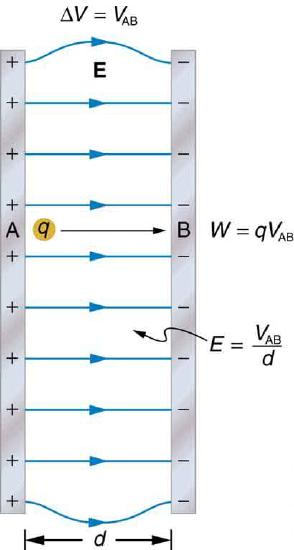
\includegraphics[scale=0.3]{metal_plates_v}
	\end{center}
	The work done to move the charge from the higher potential to the lower potential is:
	$$\text{W}=-\Delta \text{PE}=-q\Delta V=qV_{\text{AB}}\text{, where V}_{\text{AB}}\text{ is the potential difference between A and B}$$
	We know that the work done is given by W=Fd. Since F=qE, we see that W=qEd. Thus,
	$$\text{q}V_{\text{AB}}=\text{qEd}\text{, therefore,}$$
	$$V_{\text{AB}}=\text{Ed}$$
	Thus, for a uniform electric field, we can relate the electric field strength to the potential difference as shown above.
	\subsubsection*{Equipotential Lines \& Surfaces}
	We have seen above that potential is defined as the potential energy per unit charge. Thus, for a point source charge Q, the absolute potential at a distance r is given as follows:
	$$\text{V}=\dfrac{\text{PE}}{\text{q}}$$
	We know that the potential energy between the source charge Q and the test charge q is given by:
	$$\text{PE}=\dfrac{\text{KQq}}{\text{r}}$$
	Substituting this to the equation above, we get:
	$$\text{V}=\dfrac{\dfrac{\text{KQq}}{\text{r}}}{\text{q}}$$
	$$\text{V}=\dfrac{\text{KQ}}{\text{r}}$$
	Thus, a point charge's potential only depends on its magnitude and the distance from itself. For a positive point charge Q, we have its electric field as follows and as we are equidistant from the charge, we can infer that the potential is the same. The circle we see in the figure below is called an equipotential surface.\begin{center}
		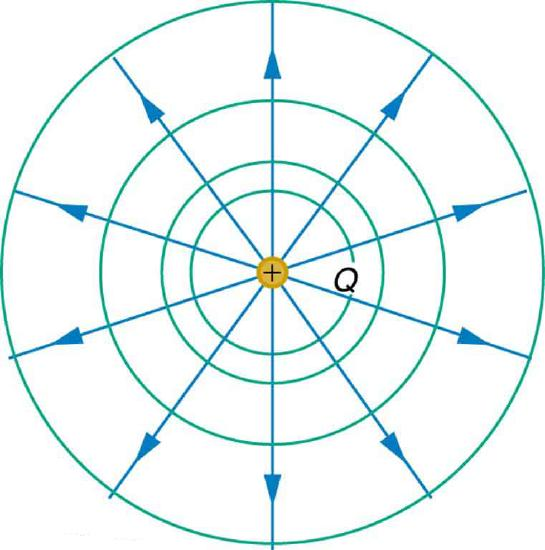
\includegraphics[scale=0.2]{equip_1}
	\end{center}
	However, as the number of charges changes, the geometry of equidistant surfaces also changes. For two charges, for example, here is the equipotential surface. We can see that it is far from being a circle. \begin{center}
		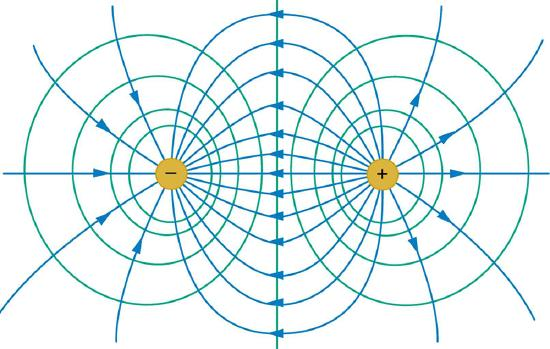
\includegraphics[scale=0.27]{equip_2}
	\end{center}
	You can also note that the equipotential surfaces are perpendicular to the electric field lines. \\ \\
	\subsubsection*{Grounding}
	A conductor is an equipotential surface in static situations. There can be no voltage difference across the surface of a conductor, or else it means that charges will flow. One of the uses of this fact is that a conductor can be fixed at zero volts by connecting it to the earth with a good conductor — a process called \textbf{grounding}. Grounding can be a useful safety tool. For example, grounding the metal case of an electrical appliance ensures that it is at zero volts relative to the earth.
	
	
\end{document}	